%----------------------------------------------------------------------------------------
%	PACKAGES AND OTHER DOCUMENT CONFIGURATIONS
%----------------------------------------------------------------------------------------


\documentclass[12pt]{article} % Default font size is 12pt, it can be changed here

\usepackage{geometry}
\geometry{left=22mm,right=22mm, top=30mm, bottom=25mm}
\usepackage{setspace} 
\usepackage{hyperref}
\usepackage[ngerman]{cleveref}

\usepackage{color,soul}

\usepackage{subfigure}


\usepackage{eurosym}

\usepackage{hhline,float}

\usepackage{fancyhdr}

\usepackage{german}

\usepackage{pdflscape}
\usepackage[utf8]{inputenc}
\usepackage[T1]{fontenc}


\usepackage{longtable}
 
\usepackage{geometry} % Required to change the page size to A4
\geometry{a4paper} % Set the page size to be A4 as opposed to the default US Letter

\usepackage{graphicx} % Required for including pictures

\usepackage{booktabs}

\usepackage{float} % Allows putting an [H] in \begin{figure} to specify the exact location of the figure
\usepackage{wrapfig} % Allows in-line images such as the example fish picture



\linespread{1.2} % Line spacing

%\setlength\parindent{0pt} % Uncomment to remove all indentation from paragraphs

\graphicspath{{Pictures/}} % Specifies the directory where pictures are stored



\begin{document}
	
	\begin{titlepage}
		
		\newcommand{\HRule}{\rule{\linewidth}{0.5mm}} % Defines a new command for the horizontal lines, change thickness here
		
		\centering % Center everything on the page
		
		\begin{figure}[h] 
			\centering
			
\includegraphics[width=.4\textwidth]{Logo-FHNW}
		\end{figure}
		
		\textsc{\Large Zwischenbericht}\\[0.5cm] % Major heading such as course name
		\begin{doublespace}
			\HRule \\[1cm]
			{ \huge \bfseries Datenübertragung mit dem Pixhawk über die UART-Schnittstelle }\\[1cm] % Title of your document
			\HRule \\[1cm]
		\end{doublespace}

		{\large 17. Oktober 2016}\\[1cm] % Date, change the \today to a set date if you want to be precise
		
		{\large Saner Kevin}\\[1cm]
		{\large Institut für Automation}
		%\includegraphics{Logo}\\[1cm] % Include a department/university logo - this will require the graphicx package
		
		\vfill % Fill the rest of the page with whitespace
		
	\end{titlepage}
	
	\pagenumbering{arabic}
	\setcounter{page}{1}
	\pagestyle{fancy}
	\lfoot{18.10.2016} %left Foot
	\cfoot{\em Projekt FindMine} %Center Foot
	\rfoot{\thepage}
	
	\section{Einleitung}
	Das folgenden Beispiel zeigt auf welche Schritte durchgeführt werden müssen um die Verbindung zum Pixhawk herzustellen, sowie was unternommen werden muss damit die Kommunikation mit Hilfe des Mavlink Protokolls hergestellt werden kann. 

	\begin{description}
		\item[Voraussetzungen:]~\par
		\begin{itemize}
			\item Ubuntu Version 14.04 oder ähnlich
			\item QGroundControl unter Linux
			\item Pixhawk inkl. sämtlicher benötigter Peripherie
			\item 2 x FTDI-Kabel 3.3V
			\item Toolchain des Single Board Computer zum Cross-Kompilieren
		\end{itemize}
	\end{description}
	
	
	\section{Ubuntu}
	Als Host-Computer wird am besten ein Computer mit Ubuntu 14.04 oder einem ähnlichen Betriebssystem eingesetzt. So gestaltet sich auch die Herstellung der Verbindung zum Pixhawk am einfachsten. Wird ein dabei ein SBC von Phytec eingesetzt empfiehlt es sich alle Arbeitsschritte mit dem mitgelieferten Betriebssystem durchzuführen. Beim eingesetzten Betriebssystem muss sichergestellt werden, dass das Package "`screen"' installiert ist. Ist dieses Package noch nicht vorhanden kann es mit dem untenstehenden Befehl nachinstalliert werden. Dieses Package wird benötigt um auf die Pixhawk-Konsole zugreifen zu können (siehe :\\
	\\
	\noindent\hspace*{30mm} \textbf{Command:} \$ sudo apt-get install screen
	
	\section{QGroundControl}
	Um den Pixhawk in Betrieb zu nehmen muss auf dem Host-Computer ebenfalls die Applikation QGroundControl vorhanden sein. Die App kann als Imagedatei von \href{https://donlakeflyer.gitbooks.io/qgroundcontrol-user-guide/content/download\_and\_install.html}{QGroundControl} heruntergeladen werden, was dessen Installation relativ einfach macht. Die heruntergeladene Datei sollte nun an sicheren Ort kopiert werden. Anschliessend müssen noch die Benutzerrechte geändert werden.
	\\
	\noindent\hspace*{30mm} \textbf{Command:} \$ chmod +x ./QGroundControl.AppImage\\
	\\
	Dieser Befehl gibt dem momentanen Benutzer die Erlaubnis die Applikation auszuführen. Der folgende Befehl wiederum führt die Applikation schliesslich aus (oder doppelklicken).\\
	
	\noindent\hspace*{30mm} \textbf{Command:} \$ ./QGroundControl.AppImage\\
	
	\section{Inbetriebnahme des Pixhawk}
	
	\subsection{Hardware}
	Bevor der Pixhawk ein erstes mal an der Computer angeschlossen werden kann, muss er zuerst entsprechend verkabelt werden. Denn einige Peripheriegerät sind zwingend notwendig für den Betrieb. Zur benötigten Peripherie gehören das GPS-Modul, der Taster sowie der Buzzer. Als Stromversorgung kann auch das mitgelieferte USB-Kabel verwendet werden, allerdings muss darauf geachtet werden, dass der verwendete USB-Port am Host-Computer die benötigte Spannung liefern kann. Für mehr Info: \href{https://3dr.com/wp-content/uploads/2014/03/pixhawk-manual-rev7.pdf}{QUICK START GUIDE}
	
	\begin{figure}[H]
		\centering
		\fbox{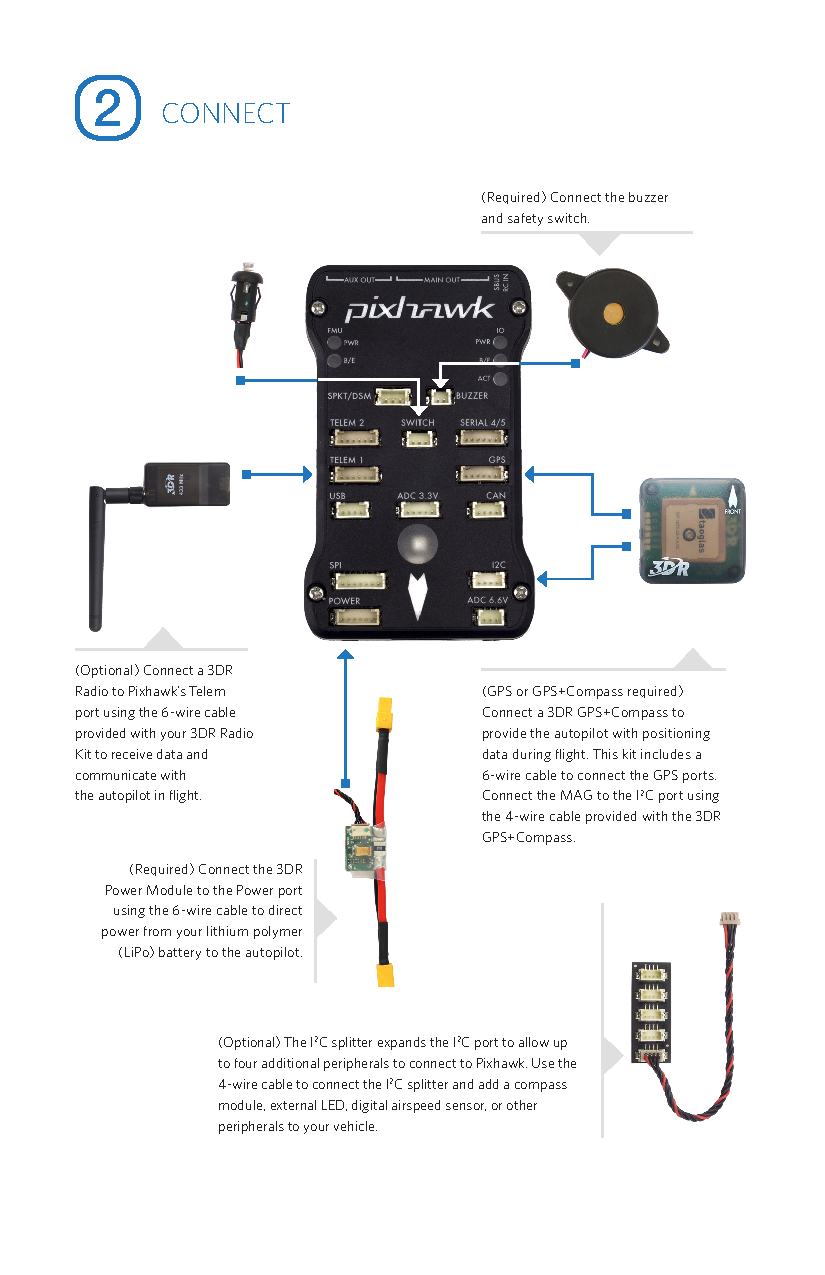
\includegraphics[scale=0.75]{connect}}
		\caption{Verkabelung des Pixhawk}
		\label{2}
	\end{figure}
	
	\subsection{Software}
	Der Pixhawk ist nun Betriebsbereit. Um nun die Sensoren zu kalibrieren wird empfohlen zuerst ein Firmwareupdate durchzuführen. Dabei wird auch die später benötigte Mavlink-Anwendung installiert. Es ist darauf zu achten, dass die PX4-Firmware und nicht die ArduPilot-Firmware geladen wird. Nachdem die Firmware erfolgreich installiert wurde, müssen die Sensoren kalibriert sowie auch der Airframe ausgewählt werden. 
	\\ \\
	QGroundControl führt dabei selbständig durch die Kalibration. Die Kalibration dient in erster Linie dazu die Maximalwerte der Beschleunigungssensoren zu bestimmen um die Lage des Pixhawk zu definieren.
	\\ \\
	Um schliesslich überprüfen zu können ob alle Systeme einwandfrei funktionieren empfiehlt es sich den Pixhawk unter freiem Himmel in Betrieb zu nehmen, denn nur so kann garantiert werden, dass GPS und Kompass exakte Daten liefern. War die Inbetriebnahme erfolgreich wird nun die aktuell Position des Pixhawks sowie die Ausrichtung in der QGroundControl-Applikation angezeigt, die Status-LED pulsiert dabei grün.
	
	
	\section{Mavlink}
	Um Daten auf den Pixhawk zu senden bzw. zu empfangen wird das Kommunikationsprotokoll Mavlink (Micro Air Vehicle Communication Protocol) verwendet. Mavlink sendet dabei C-structs über eine serielle Schnittstelle zu einer Kontrollstation. Als Kontrollstation kann zum Beispiel die vorher schon erwähnte Software QGroundControl dienen.
	\\Ziel der folgenden Arbeitsschritte ist es, die Mavlink-Messages mit einem C++-Programm interpretieren zu können. Diese Messages sollen dabei einerseits vom Host/Computer interpretiert werden können, in einem zweiten Arbeitsschritt soll das Programm aber für einen Phytec Single Board Computer kompiliert werden, damit dieser die Datenakquisition durchführen kann. 
	
	\subsection{Verkabelung}

	Um nun Daten vom Pixhawk auslesen zu können muss der Pixhawk zuerst entsprechend verkabelt werden. Erst durch diesen Schritt wird es möglich auf die Konsole des Pixhawk zuzugreifen. Wichtig ist dabei, dass ein 3.3V-Kabel verwendet wird und kein 5V-Kabel. Wahlweise kann der Pixhawk mit dem mitgelieferten USB-Kabel oder einer anderen Quelle mit Strom versorgt werden. Die Verkabelung muss nach folgendem Schema vorgenommen werden:\\
\begin{description}
	\item \textbf{Verkabelung Konsole:}\\ \\
	\begin{tabular}{p{2cm}p{4cm}p{2cm}p{4cm}}
		\centering 
		\textbf{ Pixhawk} & \textbf{(Serial 4/5)} & \textbf{FTDI}& \\ \hline
		1 & +5V (red)	& 		& N/C				\\ \hline
		2 & S4 Tx	 	&		& N/C				\\ \hline
		3 & S4 Rx		&		& N/C				\\ \hline
		4 & S5 Tx		& 5		& FTDI RX (yellow)	\\ \hline
		5 & S5 Rx		& 4		& FTDI TX (orange)	\\ \hline
		6 & GND			& 1		& FTDI GND (black)	\\ \hline
		
	\end{tabular}
\end{description}

Im folgenden Bild wird dies auch noch grafisch dargestellt:

	\begin{figure}[H]
		\centering
		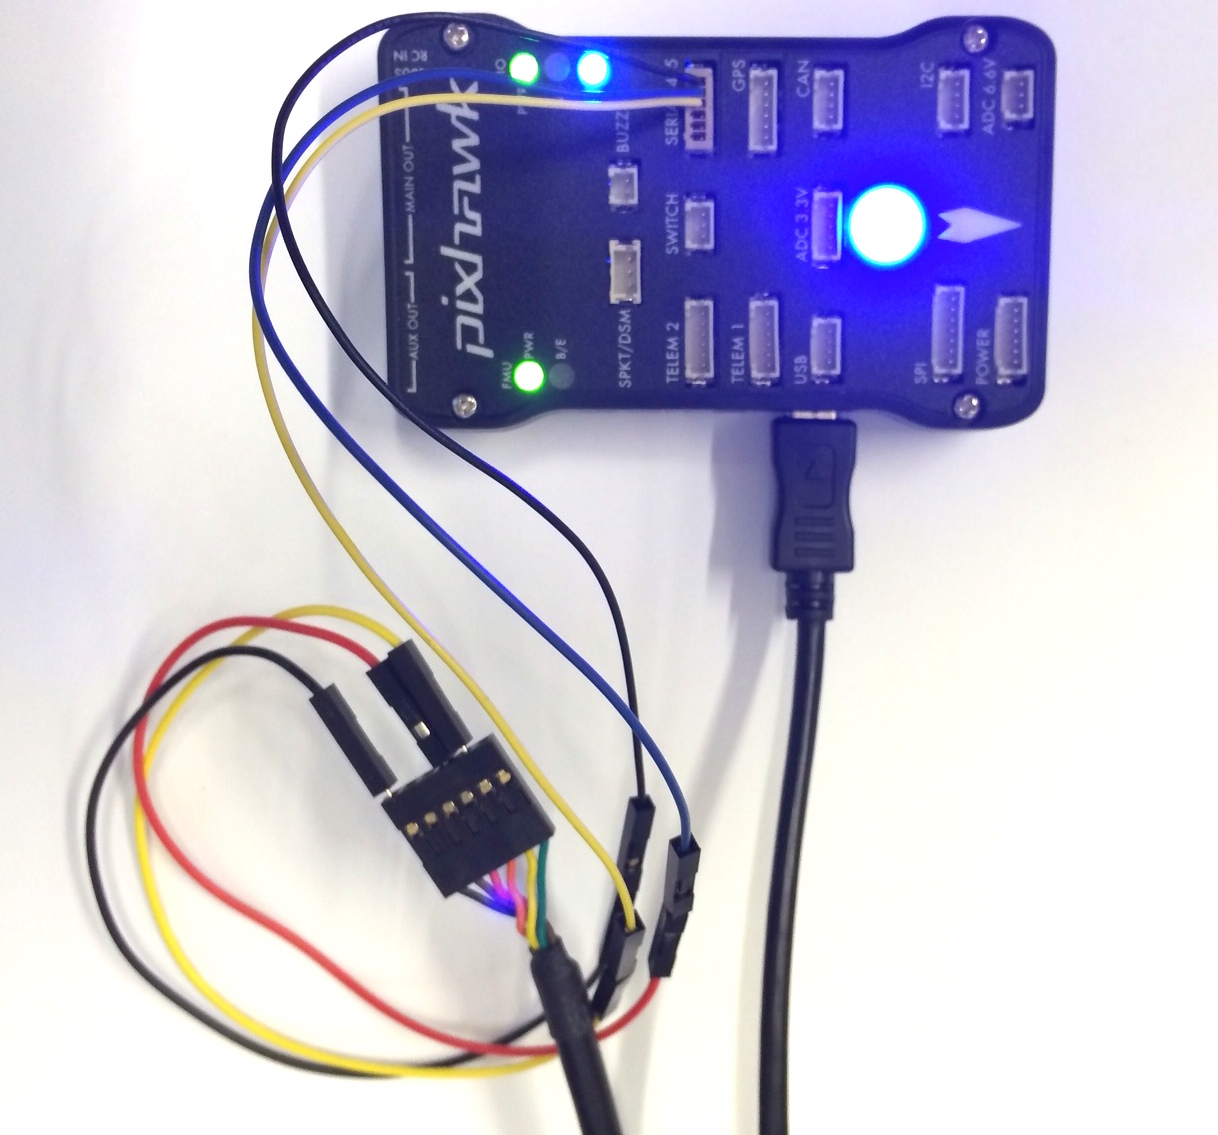
\includegraphics[scale=0.3]{Verkabelung_Mav}
		\caption{Verkabelung der Konsole}
		\label{2}
	\end{figure}
	
	\begin{description}
		\item \textbf{Verkabelung Mavlink-Kanal:}\\ \\
		\begin{tabular}{p{2cm}p{4cm}p{2cm}p{4cm}}
			\centering 
			\textbf{ Pixhawk} & \textbf{Telem 2}& \textbf{FTDI}& \\ \hline
			1 & +5V (red)	& 		& N/C				\\ \hline
			2 & Tx (out)	& 5		& FTDI RX (yellow)				\\ \hline
			3 & Rx (in)		& 4		& FTDI TX (orange)				\\ \hline
			4 & CTS (in)	& 		& N/C	\\ \hline
			5 & RTS (out)	& 		& N/C	\\ \hline
			6 & GND			& 1		& FTDI GND (black)	\\ \hline
			
		\end{tabular}
	\end{description}
	
	Im folgenden Bild wird dies auch noch grafisch dargestellt:
	
	\begin{figure}[H]
		\centering
		\subfigure[]{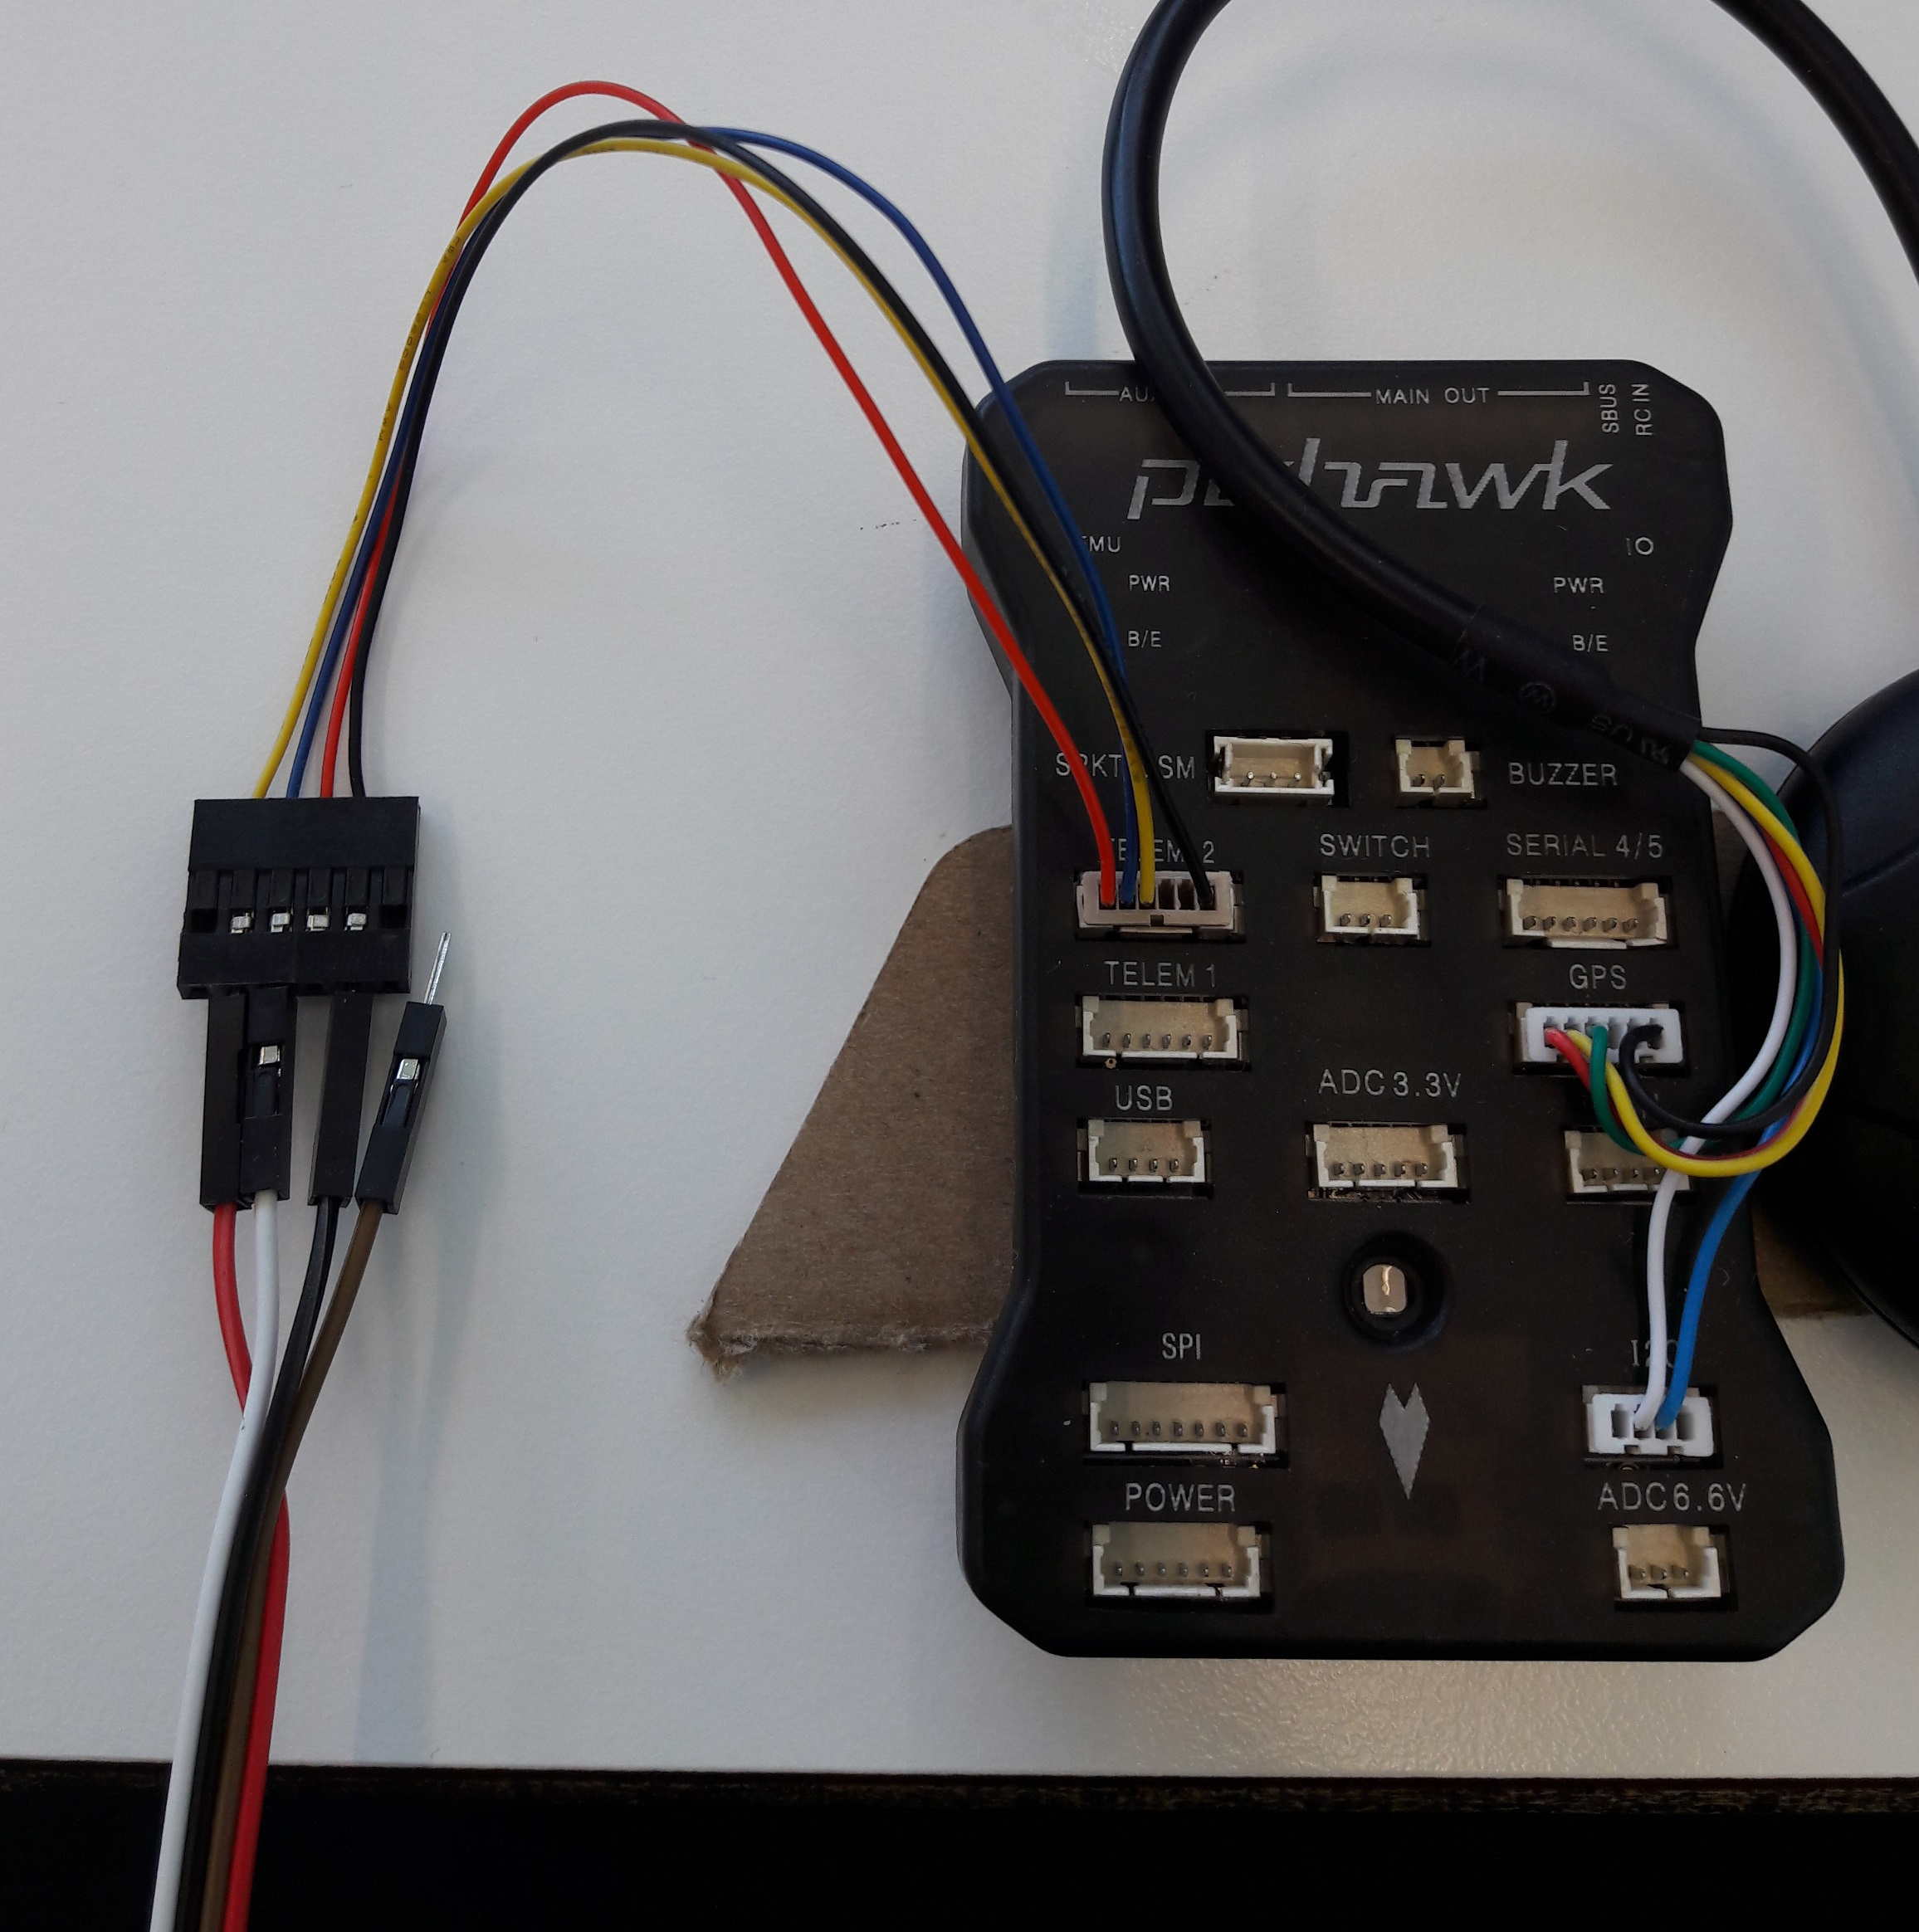
\includegraphics[scale=0.08]{PX_FTDI2}}\hfill
		\subfigure[]{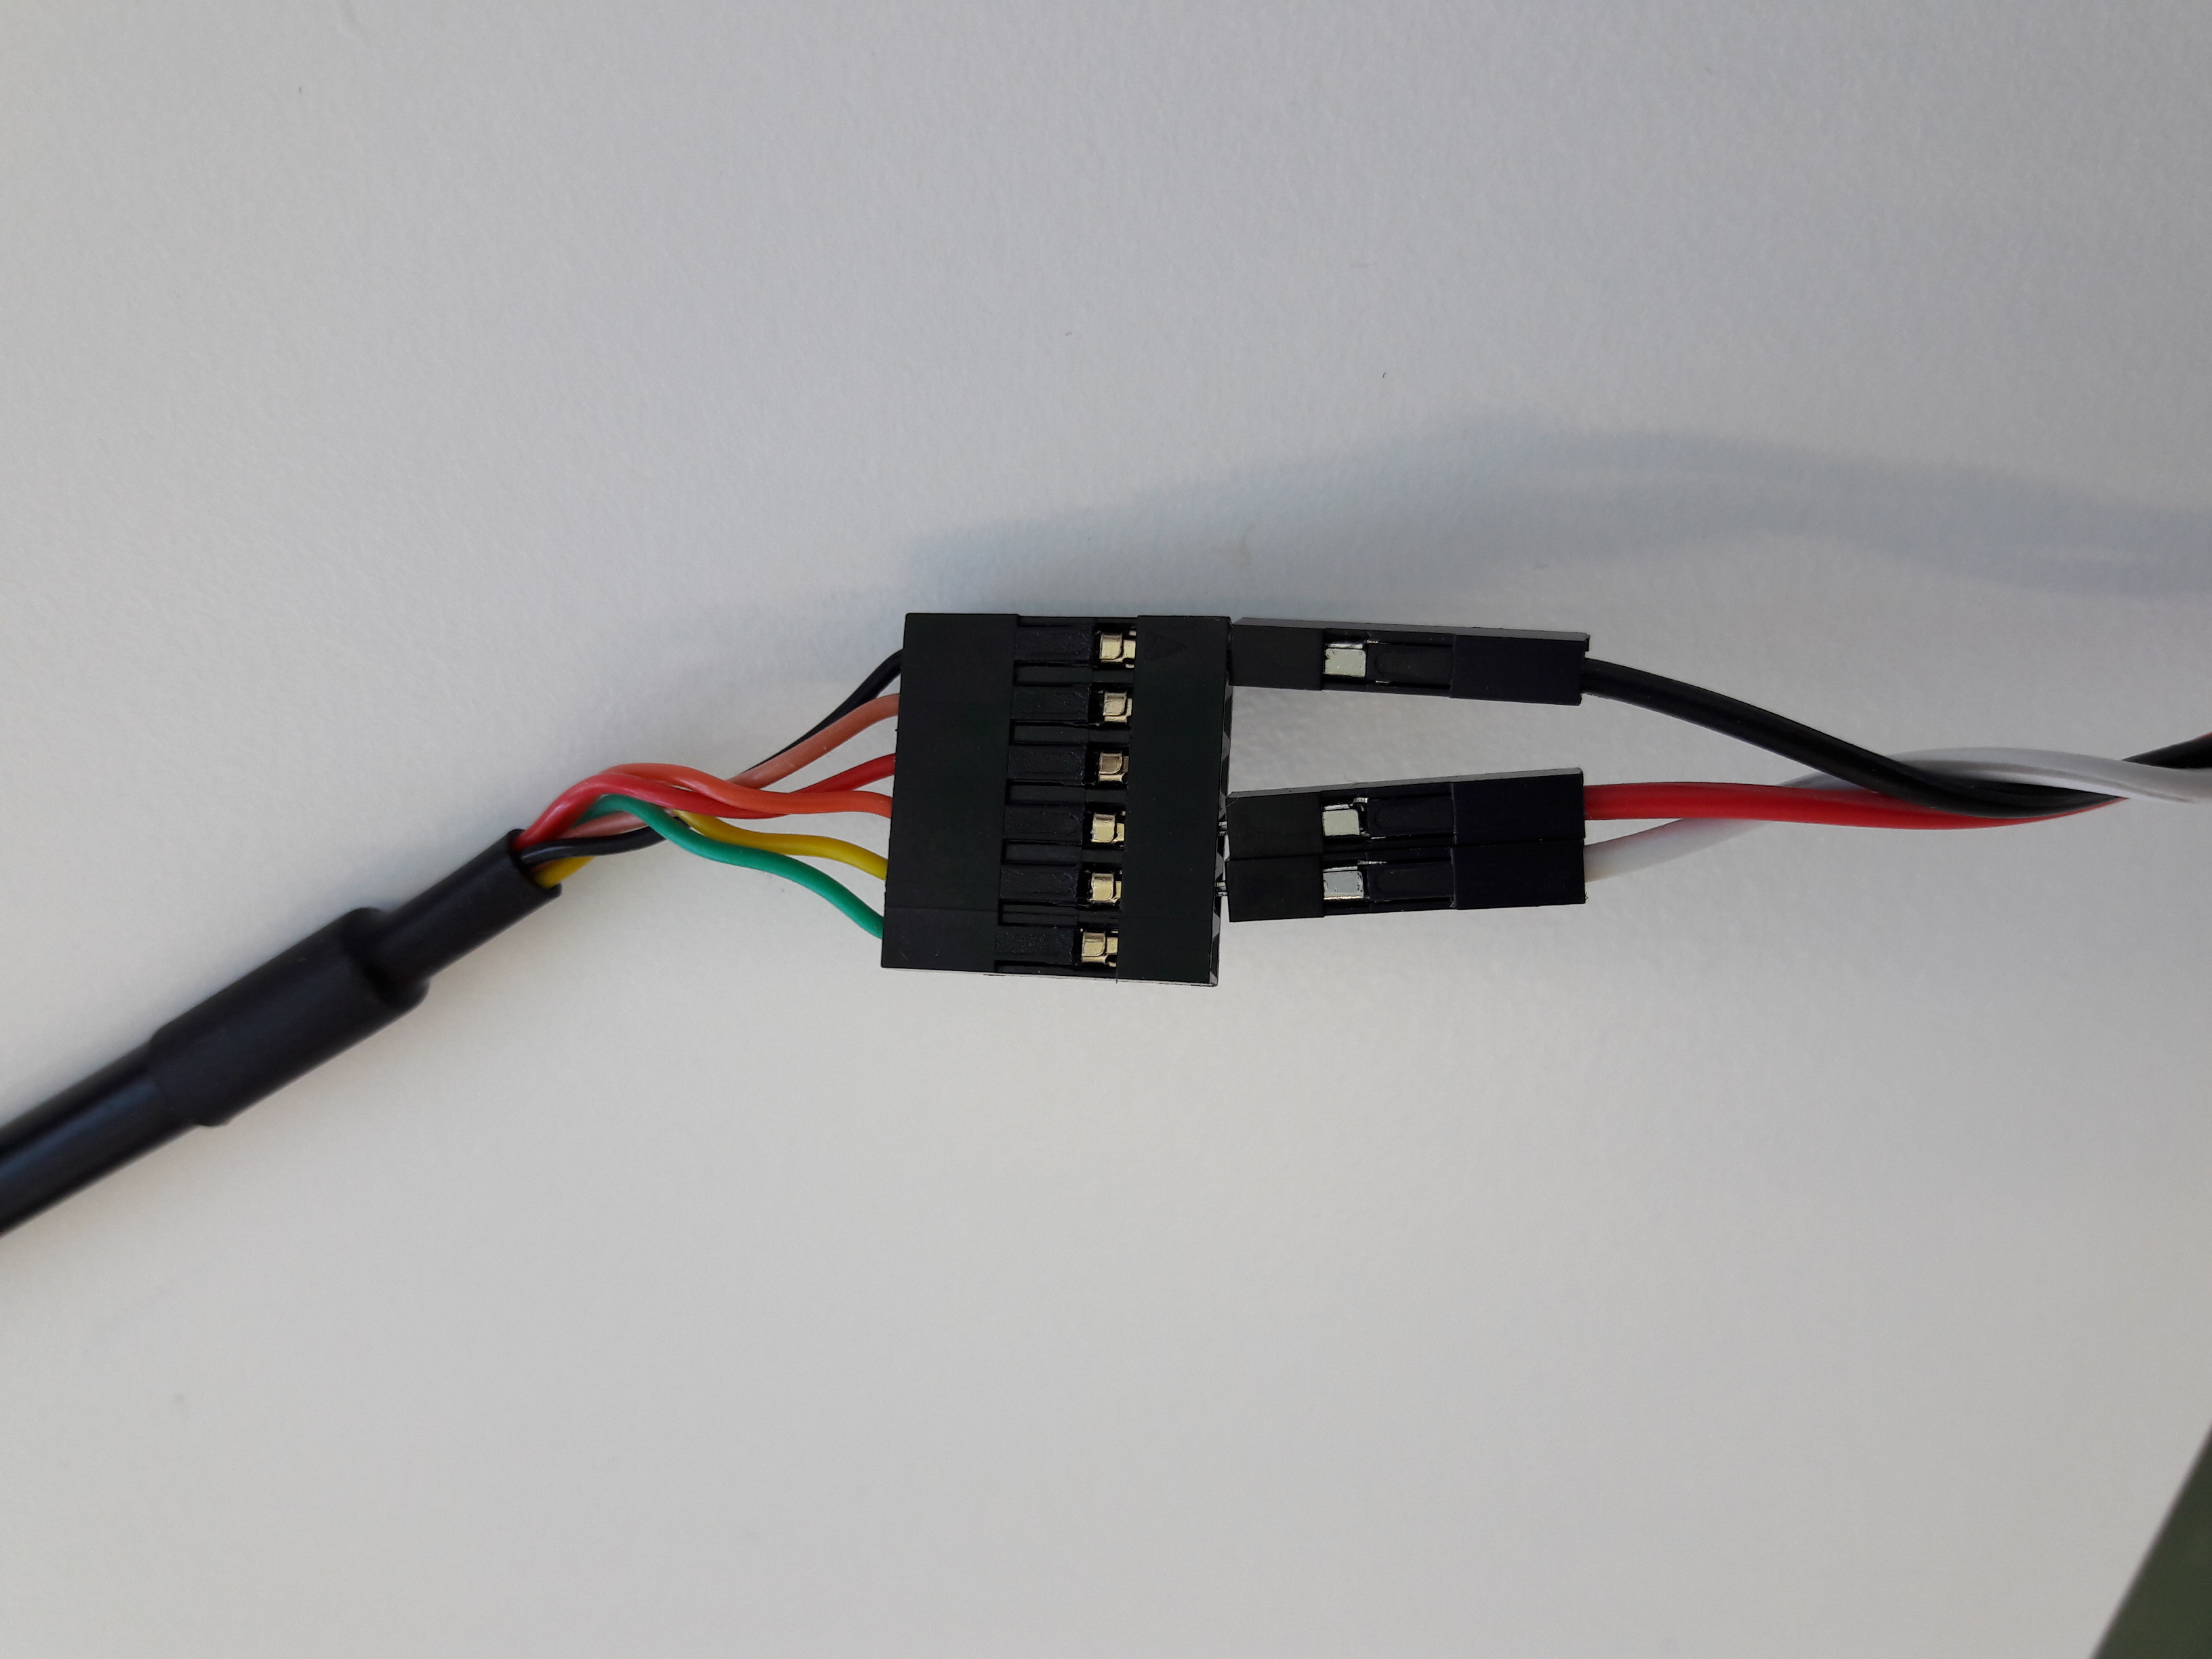
\includegraphics[scale=0.07]{PX_FTDI}}
		\caption{Verkabelung der Mavlink-Schnittstelle}
		\label{2}
	\end{figure}
	
	\noindent
	Kann der Telemetry-Port nicht verwendet werden, kann auch der serielle Port 4 verwendet werden. Dazu muss das FTDI-Kabel an die S4-Schnittstelle des Pixhawk angeschlossen werden (siehe Verkabelung Konsole).
	
	\subsection{Setup} \label{Setup}
	
	Sind sämtliche Kabel angebracht entsteht folgendes Setup:
	
	\begin{figure}[H]
		\centering
		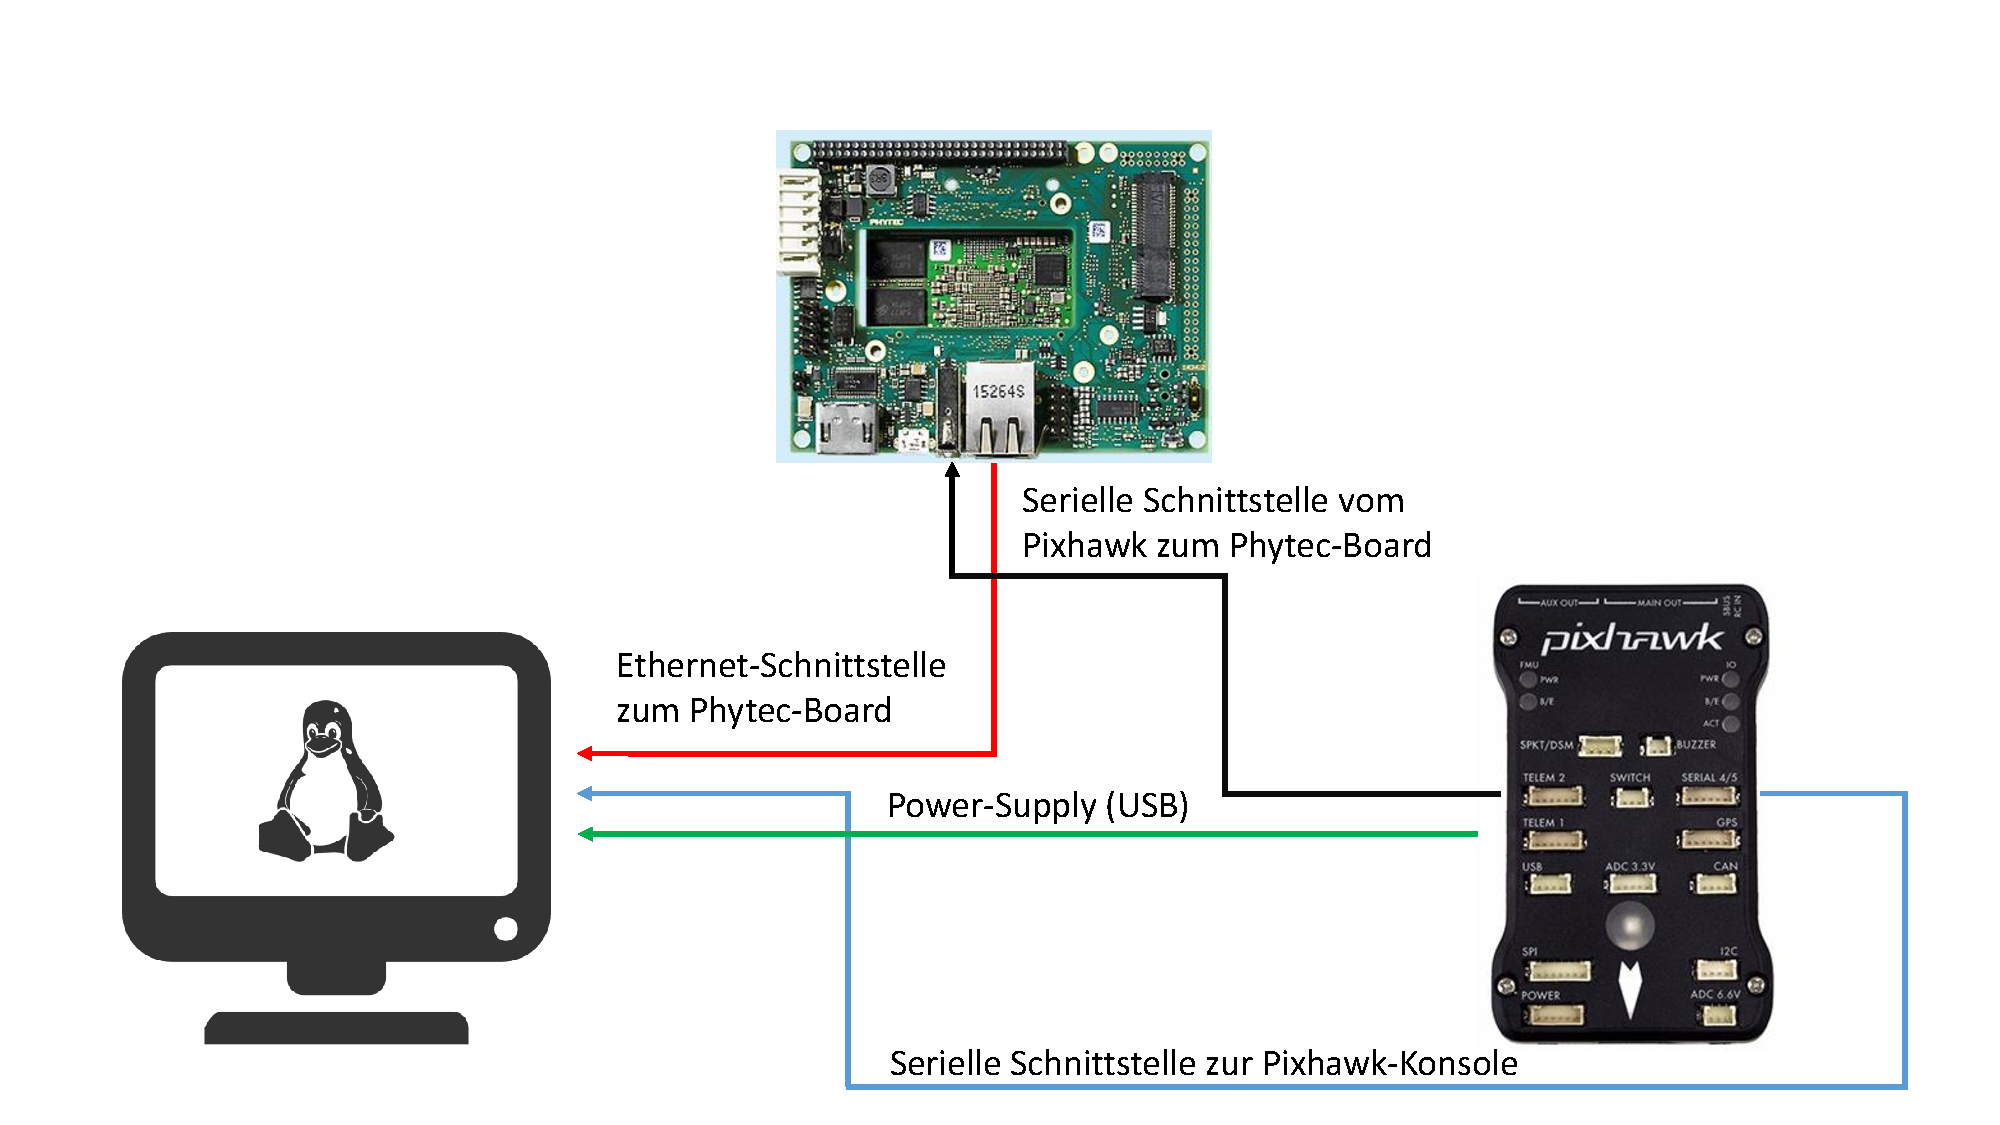
\includegraphics[scale=0.7]{Setup}
		\caption{Verkabelung des Pixhawk}
		\label{2}
	\end{figure}
	
	\subsection{Test des Setups}
	
	Der Anwender sollte nun in der Lage sein, sich auf die Konsole des Pixhawks einzuloggen. Dazu muss folgender Befehl eingetippt werden:\\
	\\
	\noindent\hspace*{30mm} \textbf{Command:} \$ screen /dev/ttyUSB0 57600 8N1\\
	\\		
	Falls der Port-Name nicht gefunden wird, kann mit dem Befehl:\\
	\\
	\noindent\hspace*{30mm} \textbf{Command:} \$ ls /dev/ttyUSB*\\
	\\
	nach allen verfügbaren Ports gesucht werden. Der Anwender ist nun über die serielle Schnittstelle auf dem Pixhawk eingeloggt.\\
	\\
	Nun kann die Stromversorgung zum Pixhawk unterbrochen werden, damit dieser neu startet. Dabei werden unter anderen sämtliche Ports ausgegeben, auf welchen Mavlink empfangen werden kann. Ist der gewünschte Port nicht dabei, kann eine entsprechende Mavlink-Session über den jeweiligen Port wie folgt gestartet werden.\\
	\\
	\noindent\hspace*{30mm} \textbf{Command:} \$ nsh> mavlink start -d /dev/ttyACM0\\
	\\
	Über welche Ports eine aktive Mavlink-Session läuft ist von Bedeutung wenn versucht wird die gesendeten Daten entgegen zu nehmen und zu verarbeiten. Das folgende Beispiel zeigt einen Ausschnitt des Start-up-Prozederes des Pixhawks, daraus ist ersichtlich über welche Ports Mavlink-Messages gesendet bzw. empfangen werden.
	
		\begin{figure}[H]
			\centering
			\fbox{\includegraphics[trim = 22mm 240mm 30mm 22mm, clip, scale=0.75]{Mavlink_Out}}
			\caption{Programm Output}
			\label{2}
		\end{figure}
	
	\subsubsection{C++-Mavlink-Schnittstelle}
	
	Das Programm welches verwendet wird ist auf \href{https://github.com/mavlink/c_uart_interface_example}{GitHub} frei verfügbar. Die entsprechenden Files können mit dem Befehl:
	\\ \\
	\noindent\hspace*{15mm} \textbf{Command:} \$ git clone https://github.com/mavlink/c\_uart\_interface\_example.git\\ \\
	\noindent
	auf dem Host-Computer kopiert werden. Nun muss das Programm erst einmal kompiliert werden. Um das Programm sowie die Verbindungen zum Pixhawk zu testen sollte das Programm zuerst lokal kompiliert werden (ohne Cross-Compiler). Der folgende Befehl kompiliert das Programm zu einem Binary:
	\\ \\
	\noindent\hspace*{30mm} \textbf{Command:} \$ cd /path/to/directory/c\_uart\_interface\_example\\
	\noindent\hspace*{30mm} \textbf{Command:} \$ make\\
	\\
	Der Befehl "`make"' hat nun mithilfe der, im Verzeichnis vorhandenen "`Makefiles"' ein Executable erstellt. mit welchen bereits getestet werden kann ob, die Verkabelung funktioniert und ob der Pixhawk korrekt initialisiert wurde.\\
	Um das eben erstellt Programm zu starten muss der folgende Befehl ausgeführt werden:
	\\ \\
	\noindent\hspace*{30mm} \textbf{Command:} \$ ./mavlink\_control -d /dev/ttyACM0\\ \label{Exec Mav}
	\\
	Sieht der Output dabei wie folgt aus konnte die Verbindung erfolgreich hergestellt werden.
	\begin{figure}[H]
		\centering
		\fbox{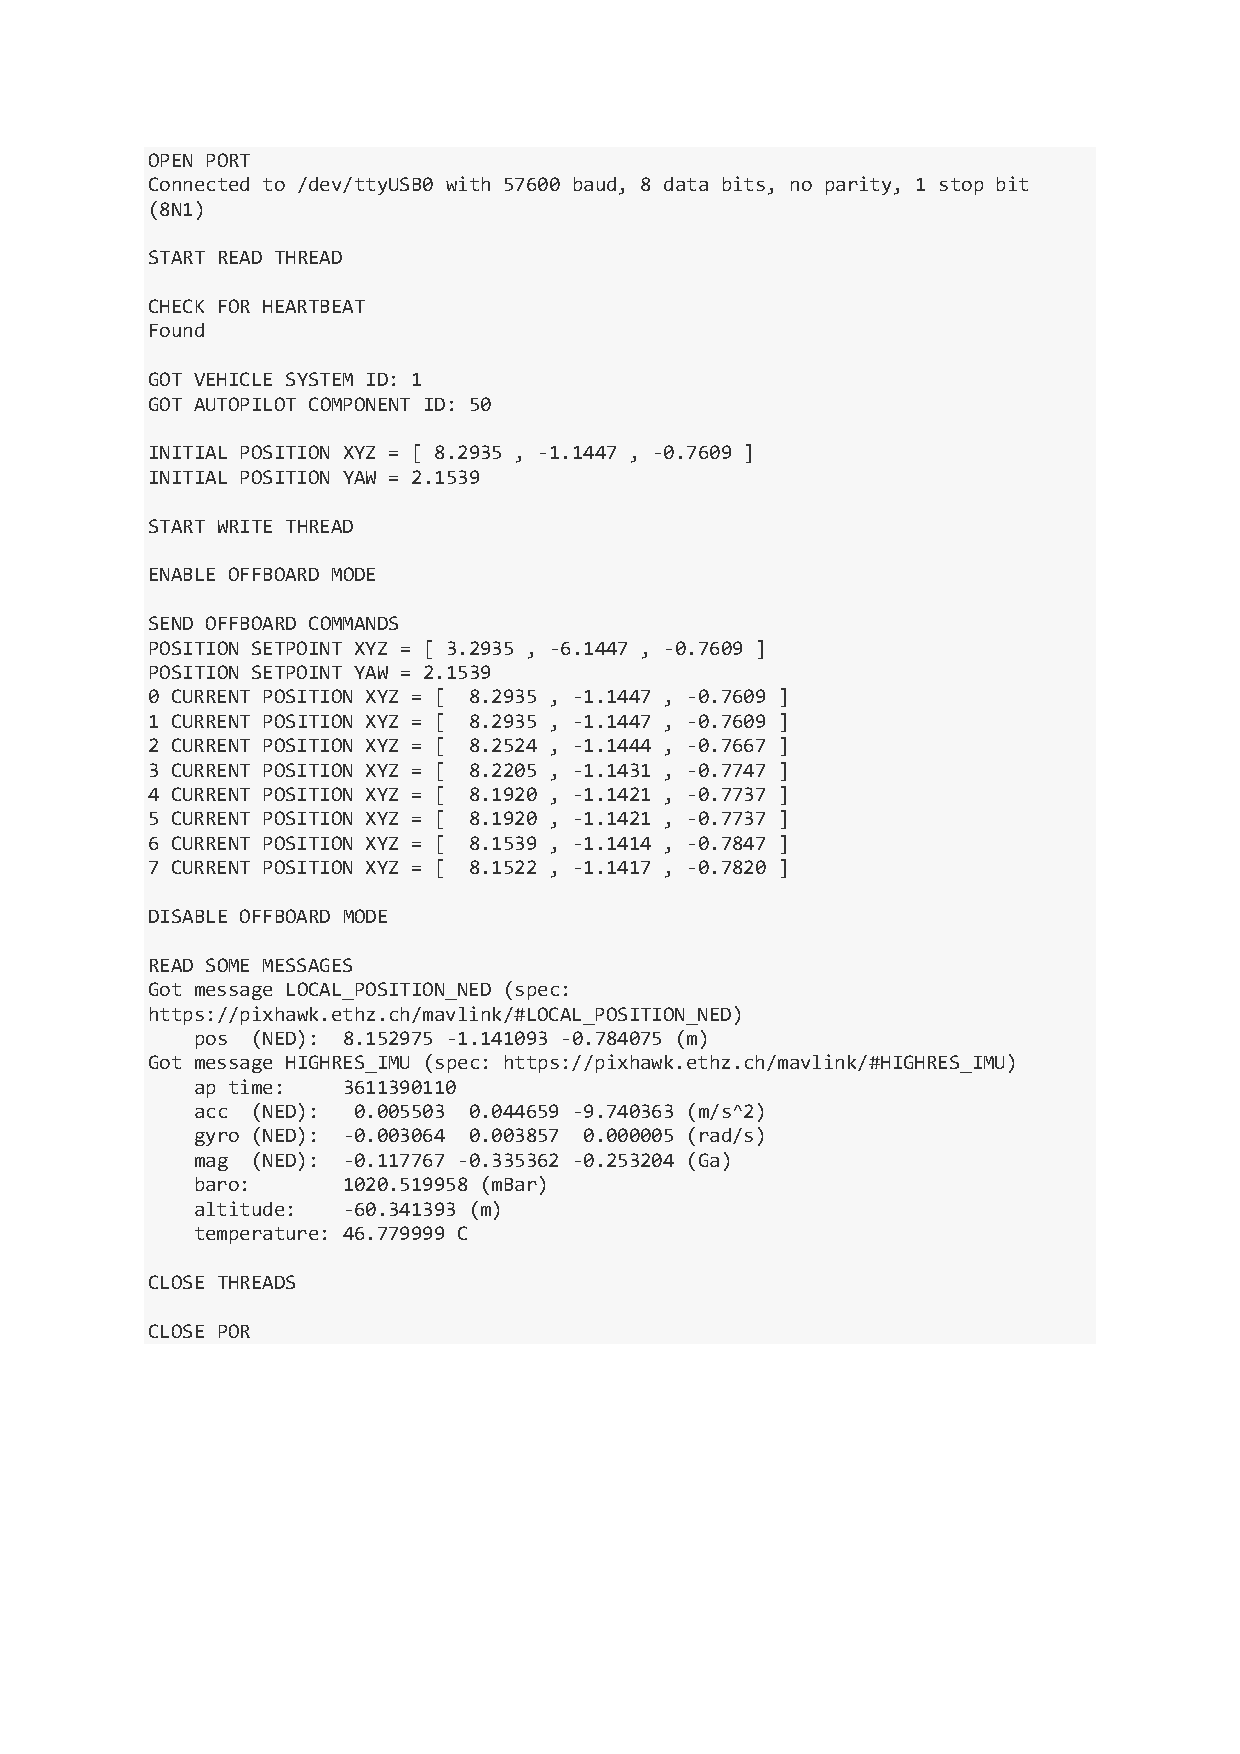
\includegraphics[trim = 20mm 70mm 30mm 20mm, clip, scale=0.65]{Mavlink_Example}}
		\caption{Programm Output}
		\label{2}
	\end{figure}
	\noindent
	Der Port "`ttyACM0"' entspricht dabei dem USB-Port des Pixhawk, um nun auch die serielle Verbindung über das FTDI-Kabel zu testen muss der Mavlink-Port (Device: -d) zu "`ttyUSB*"' geändert werden. Ist der Output derselbe funktioniert auch diese Verbindung.
	
	\subsection{Cross-Compiling}
	
	Da der Phytec Single Board Computer über eine andere Architektur verfügt als ein normaler Desktop-Computer muss das Programm speziell dafür kompiliert werden. Der Phytec verfügt über die, für embedded Systeme, typische ARM-Architektur. Alle benötigten Tools für das Cross-Compiling sind dabei auf dem mitgelieferten USB-Stick.
	
	\subsubsection{Eclipse}
	Da die Entwicklungsumgebung Eclipse bereits auf dem Phytec USB-Stick vorhanden ist, empfiehlt es diese auch zu verwenden. Eine Anleitung wie diese für das Entwickeln von C-Programmen konfiguriert werden muss, befindet sich ebenfalls auf dem USB-Stick (Application Guide). Um zu überprüfen, ob die Toolchain und der Compiler korrekt funktionieren sollte zuerst ein einfaches C-Programm erstellt werden. Eine komplette Anleitung um ein "`Hello World"' in C zu entwickeln findet man dabei im "`Application Guide"' (S. 10 - 23) von Phytec.
	
	\subsubsection{C++-Compiling}
	Das zu kompilierende Mavlink-Interface wurde dabei in C++ geschrieben, was es um einiges komplizierter macht dieses zu kompilieren. Die folgende Anleitung soll Schritt für Schritt aufzeigen was unternommen werden muss, um ein auf dem Phytec lauffähiges Executable des Mavlink-Interfaces zu erhalten.
	
	\paragraph*{Projekt erstellen:}
	Für die Entwicklung eines C++-Programms muss in Eclipse ein neues C++-Projekt erstellt und benannt werden. Ein leeres Projekt ist dabei am besten geeignet.
	
	\paragraph*{Build-Pfade:}
	Damit für das Mavlink-Interface sämtliche Header-Files zur Verfügung stehen, muss das entsprechende Verzeichnis im Projekt miteinbezogen werden. Mit "rechts-klicken" auf das Projekt können unter "`Properties -> C/C++Build -> Settings -> Includes"' Build-Pfade  zum Projekt hinzugefügt werden. Für das Mavlink-Interface muss das Verzeichnis "`/path/to/dir/mavlink/include/mavlink/v1.0"' hinzugefügt werden.
	
	\paragraph*{C++-Files:} 
	Als nächster Schritt können alle C++-Files zum Projekt hinzugefügt werden. Die, für das Mavlink-Interface, benötigten Files sind "`autopilot\_interface.cpp"', "`mavlink\_control.cpp"' und "`serial\_port.cpp"' und deren Header-Files. Treten dabei keine Fehler in den C++-Files auf, ist dies ein Zeichen dafür, dass bis zu diesem Schritt alles richtig gemacht wurde.
	
	\paragraph*{Konfiguration:}
	Da das Mavlink-Interface-Programm ein sogenanntes "`multithreaded"' Programm ist, muss die Bibliothek "`pthread"' ins Programm eingebunden werden. Dazu muss unter "`Properties -> C/C++ Build -> Settings -> GCC C++ Linker -> Libraries"' "`pthread"' hinzugefügt werden.\\
	\\
	Die Konfiguration des "`GCC C Compiler"' erfolgt gleich wie zur Entwicklung von C-Programmen. Als "`Command"' muss lediglich \$\{CC\} eingegeben werden. Auf die gleiche Art kann auch der "`GCC C++ Compiler"' konfiguriert werden.\\
	\\
	Als Linker kann jedoch nicht der GCC-Linker verwendet werden. Dazu muss ein G++-Linker verwendet werden. Dazu muss der komplette Pfad des Linker eingebunden werden. Somit muss zuerst nach dem G++-Compiler gesucht werden. Das gesucht File heisst "`arm-phytec-linux-gnueabi-g++"' und befindet sich normalerweise im Ordner "`/opt/yogurt/iMX6-PD15.2.0/sysroot/x86\_64-yogurtsdk-linux/usr/bin/arm-phytec-gnueabi"'. Wie im "`Application Guide"' beschrieben muss auch hier in den Linker-Settings \$\{LDFLAGS\} ergänzt werden.\\
	\\
	Als letztes muss auch noch der "`GCC Assembler"' konfiguriert werden. Dazu muss auch lediglich, wie im "`Application Guide"' beschrieben, unter "`Command"' \$\{AS\} eingegeben werden.\\
	\\
	Nun sollte durch "`Build Project"' erfolgreich ein Binary (Executable) hergestellt werden können.
	
	\paragraph{Post-build:}
	Um das Programm sogleich auf dem Phytec ausführen zu können, können die Post-build steps so konfiguriert werden, dass das erstellt Executable sogleich auf den Phytec geladen und ausgeführt wird. Dazu muss folgendes Command ergänzt werden: "`scp ./NameOfExec root@192.168.3.11:/. ;ssh root@192.168.3.11 /NameOfExec"'. Das Executable wird so im Root-Verzeichnis des SBCs ausgeführt.\\
	\\
	\textbf{Achtung:} Die Netzwerkumgebung muss natürlich zuerst richtig konfiguriert werden, damit die Post-build steps korrekt ausgeführt werden.
	
	\newpage
	\paragraph{Konfiguration Phytec:}
	Wird zum ersten Mal versucht das erstellte Executable auszuführen, wird wahrscheinlich eine Fehlermeldung angezeigt. Nämlich dass das File nicht gefunden wird. Diese Fehlermeldung wird ausgegeben da der zum Ausführen des Programms benötigte Interpreter nicht gefunden wird. Der Name des benötigten Interpreters erfährt man durch die folgende Befehlszeileneingabe:\\
	\\ 	
	\noindent\hspace*{30mm} \textbf{Command:} \$ readelf -l NameOfExec\\
	\\
	Damit das Programm ausgeführt werden kann, muss das in der Zeile "`Requesting program interpreter"' File im richtigen Verzeichnis vorhanden sein. Sucht man dieses File auf dem Phytec SBC wird man feststellen, dass dieses nicht vorhanden ist. Allerdings existiert ein File mit einem ähnlichen Namen, wie zum Beispiel "`ld-linux-armhf.so.3"'. Dies ist der auf dem Phytec vorhandene Interpreter oder zumindest zeigt dieses File auf den Interpreter. Um nun den Interpreter dem erstellten Programm zugänglich zu machen muss ein \href{https://de.wikipedia.org/wiki/Symbolische\_Verkn\%C3\%BCpfung}{symbolischer Link} erstellt werden, der auf das File "`ld-linux-armhf.so.3"' zeigt. Der Link kann wie folgt erstellt werden:
	\\ 	
	\noindent\hspace*{30mm} \textbf{Command:} \$ ln -s /lib/ld-linux-armhf.so.3 /lib/ld-linux.so.3\\
	\\
	Nun sollte das erstellte Programm ausgeführt werden können.

	
	\subsubsection{Ergebnis}
	Nach dem Post-build wird das erstellte Programm auf dem Phytec ausgeführt, jedoch, in der Regel, sogleich wieder durch eine Exception abgebrochen. Die passiert weil das Standard-Device (/dev/ttyUSB0) nicht verfügbar ist. Ist jedoch die erste Programmzeile "`OPEN PORT"' sichtbar, ist das Programm lauffähig. Nun muss lediglich der Pixhawk wie in Kapitel \pageref{Setup}.2 erklärt an den SBC angeschlossen werden. Somit können der Pixhawk und der Phytec SBC nun über Mavlink kommunizieren, dass heisst es können Kommandos gesendet wie auch empfangen werden.\\
	\\
	Das Programm kann nach der korrekten Verkabelung auf dem Phytec SBC ausgeführt werden, dazu kann derselbe Befehl wie beim Starten vom Host-Computer verwendet werden (siehe \pageref{Exec Mav}). Ist der Programmoutput ebenfalls derselbe wie unter bei Abb. \ref{2} wurde das Setup richtig erstellt so wie sämtliche Schritte zur Kompilation des Programms korrekt ausgeführt. 
	
	
	
	
	
	

\newpage
\renewcommand\refname{Literaturverzeichnis}
\begin{thebibliography}{99} % Bibliography - this is intentionally simple in this template
	\raggedright
	
	\bibitem{Prosys}
	Prosys OPC UA Java SDK:
	\newblock {\em Preisliste}
	\newblock [online] Available at: https://downloads.prosysopc.com/opcua/Prosys\_OPC\_UA\_Java\_SDK\_Price\_List.pdf [Zugriff am 21.06.2016]

\end{thebibliography}

	
\end{document}